\documentclass{article}
\usepackage{epsfig, latexsym}

\begin{document}

\newcommand{\SOPmin}{${\rm SOP}_{\rm min} \ $}
\newcommand{\POSmin}{${\rm POS}_{\rm min} \ $}
\newcommand{\bs}{\backslash}
\newcommand{\x}{\addtocounter{enumi}{1} \theenumi}


\title{
\Huge{CSE 271}\\
\normalsize{Exam 3}\\
\normalsize{Return this document!!!}\\
\makebox[4in][l]{Name:}
Student ID:}
\date{}

\maketitle{}

\begin{enumerate}
\item {\bf (3 pts.)} How many different \SOPmin realizations does 
F(A,B,C,D)=$\Sigma$m(3,4,5,6,7,8,9,11,12) have?  That is, how many 
different, correct solutions can you find for the kmap?

$$ \begin{array} {c||c|c|c|c}
        AB \bs CD & 00 & 01 & 11 & 10 \\ \hline \hline
        00        &    &    &    &    \\ \hline
        01        &    &    &    &    \\ \hline
        11        &    &    &    &    \\ \hline
        10        &    &    &    &    \\
\end{array} $$ 

\begin{tabular}{p{0.75in}p{0.75in}p{0.75in}p{0.75in}p{0.75in}}
a) 1 & b) 2 & c) 3 & d) 4 & e) 5 or more \\
\end{tabular}

\item {\bf (3 pts.)} The output of a sequential circuit is fundamentally
different than a combinational circuit because the sequential circuits 
output is a function of the?
\begin{description}
\item{a) } State
\item{b) } Input
\item{c) } Output
\item{d) } Number of inputs
\item{e) } The staple monkey
\end{description}

\item {\bf (2 pts.)} You are told to implement a 3 bit counter using our seven
step FSM design process.  Each state represents the current count value.  The
state assignment is performed using a dense encoding. 
How many flip flops will this FSM require?

\begin{tabular}{p{0.75in}p{0.75in}p{0.75in}p{0.75in}p{0.75in}}
a) 3 & b) 4 & c) 7 & d) 8 & e) 16 \\
\end{tabular}

\item {\bf (2 pts.)} You are told to implement a 3 bit counter using the
ones hot design process.  Each state represents the current count value. 
How many flip flops will the counter require?

\begin{tabular}{p{0.75in}p{0.75in}p{0.75in}p{0.75in}p{0.75in}}
a) 3 & b) 4 & c) 7 & d) 8 & e) 16 \\
\end{tabular}

\pagebreak
\item {\bf (2 pts.)} Given the following state table and the state assignment,
determine the entry in the transition kmap marked with a *.
{\small
$$\begin{array}{lll}
$$\begin{array}{c||c|c}
        cs \bs X & 0   &  1  \\ \hline \hline
        A        & B,0 & A,0 \\ \hline
        B        & D,0 & A,0 \\ \hline
        C        & C,1 & B,1 \\ \hline
        D        & A,1 & C,1 \\ 
\end{array}$$
&
$$\begin{array}{c||c|c}
        state & Q_1 & Q_0    \\ \hline \hline
        A     & 1 & 0  \\ \hline
        B     & 0 & 0 \\ \hline
        C     & 1 & 1 \\ \hline
        D     & 0 & 1 \\
\end{array}$$
&
$$\begin{array}{c||c|c}
        Q_1 Q_0 \bs X & 0   &  1   \\ \hline \hline
        00       &     &     \\ \hline
        01       &     &     \\ \hline
        10       & *   &     \\ \hline
        11       &     &     \\
\end{array}$$\\
\end{array}$$}

\begin{description}
\item{a) }00,0
\item{b) }01,1
\item{c) }10,0
\item{d) }11,0
\item{e) }None of the above.
\end{description}

Given the transition kmap to the right, determine the MIEs
and OEs.
{\small
$$\begin{array}{cll}
$$\begin{array}{c||c|c|c|c}
        Q \bs X_1 X_0 & 00  & 01  & 11  & 10  \\ \hline \hline
        0             & 1,1 & 1,1 & 0,1 & 0,1 \\ \hline
        1             & 1,0 & 0,0 & 0,0 & 1,0 \\
\end{array}$$
&
$$\begin{array} {c||c|c|c|c}
        Q \bs X_1 X_0 & 00 & 01 & 11 & 10 \\ \hline \hline
        0             &    &    &    &    \\ \hline
        1             &    &    &    &    \\
\end{array}$$
&
$$\begin{array} {c||c|c|c|c}
        Q \bs X_1 X_0 & 00 & 01 & 11 & 10 \\ \hline \hline
        0             &    &    &    &    \\ \hline
        1             &    &    &    &    \\
\end{array}$$ \\
Q^+,Z & D= & Z= \\
\end{array}$$}
\item {\bf (2 pts.)} What does $D=$ ?
\begin{description}
\item{a) }$X_1'X_0' + Q'X_1' + QX_1X_0'$
\item{b) }$X_1'X_0' + Q'X_1' + QX_0'$
\item{c) }$Q'X_1' + QX_1X_0'$
\item{d) }$Q'X_1' + QX_0'$
\item{e) }$Q'$
\end{description}

\item {\bf (2 pts.)} What does $Z=$ ?
\begin{description}
\item{a) }$X_1'X_0' + Q'X_1' + QX_1X_0'$
\item{b) }$X_1'X_0' + Q'X_1' + QX_0'$
\item{c) }$Q'X_1' + QX_1X_0'$
\item{d) }$Q'X_1' + QX_0'$
\item{e) }$Q'$
\end{description}




\pagebreak
Questions 8-11 concern the FSM realization of the state diagram given below.
Assume a ones hot encoding of the states.  The input is $X$ and the output
$Z$.  Let $D_A$ be the input to the flip flop representing state $A$.  Let $Q_A$
be the output from the flip flop representing state $A$.  Apply the preceding
definitions to $D_B, Q_B, D_C, Q_C, D_R, Q_R$.

\item {\bf (1 pts.)} How many flip flops are required to realize this FSM?

\begin{tabular}{p{0.75in}p{0.75in}p{0.75in}p{0.75in}p{0.75in}}
a) 1 & b) 2 & c) 3 & d) 4 & e) 5 \\
\end{tabular}

\item {\bf (3 pts.)} What is the memory input equation for flip flop $A$?
\begin{description}
\item{a) } 1
\item{b) } 0
\item{c) } $X'Q_B$
\item{d) } $XQ_A + XQ_C$
\item{e) } None of the above.
\end{description}

\item {\bf (3 pts.)} What is the memory input equation for flip flop $R$?
\begin{description}
\item{a) } 1
\item{b) } 0
\item{c) } $XQ_B + X'Q_C$
\item{d) } $Q_R$
\item{e) } None of the above.
\end{description}
\includegraphics[-60mm,15mm][0mm,15.1mm]{./Fig3/sd.eps}
\item {\bf (3 pts.)} What is the equation for $Z$?
\begin{description}
\item{a) } 0
\item{b) } 1
\item{c) } $Q_R$ + $Q_C$
\item{d) } $XQ_R + XQ_C + XQ_B + XQ_A$
\item{e) } None of the above.
\end{description}

\pagebreak

The figure below shows a FSM constructed from 1 D flip flop
and some combinational logic.  The timing diagram to the
right shows the response of the circuit to an input sequence
$X$ applied to it.  The timing diagram shows small propagation
delays.  From the timing diagram you are to infer the contents
of the combinational logic box.

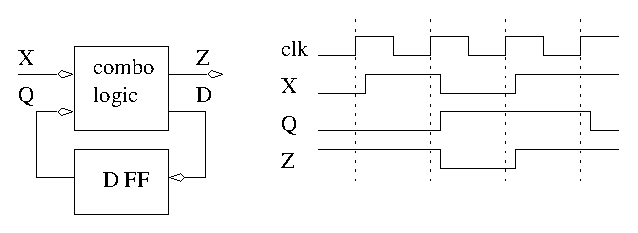
\includegraphics{./Fig3/fsm_analysis.eps}

\item {\bf (3 pts.)} Which of the following describes $D$?
\begin{description}
\item{a) } $D=Q'$
\item{b) } $D=X'Q$
\item{c) } $D=X + Q'$
\item{d) } $D=XQ'+X'Q$
\item{e) } $D$ Cannot be determined from given information.
\end{description}

\item {\bf (3 pts.)} Which of the following describes $Z$?
\begin{description}
\item{a) } $Z=Q$
\item{b) } $Z=X'Q$
\item{c) } $D=X + Q'$
\item{d) } $Z=X'Q+XQ'$
\item{e) } $Z$ Cannot be determined from given information.
\end{description}

\pagebreak
The following circuit is used to read and write a RAM.
Consult it for questions 14-16.  Note, this question
requires you to determine the direction of data flow in 
the circuit, hence arrows are not shown on the data line.
In addition you shoud not infer anything from the position
of the data lines incident to the regsiters.

\includegraphics{./Fig3/ramtsb}

\item {\bf (3 pts.)} 
Which register does the RAM read data from?

\begin{tabular}{p{1.75in}p{1.75in}}
a) RegA & b) RegB \\
\end{tabular}


\item {\bf (3 pts.)} 
For which operation does the TSB tristate its output?

\begin{tabular}{p{1.75in}p{1.75in}}
a) RAM Read & b) RAM Write \\
\end{tabular}


\item {\bf (3 pts.)} 
The address lines (not shown in the schematic) will need to 
have a TSB as well.

\begin{tabular}{p{1.75in}p{1.75in}}
a) True & b) False \\
\end{tabular}


\item {\bf (3 pts.)} What is the state table entry for the cell marked with letter Z?

\begin{tabular}{p{0.75in}p{0.75in}p{0.75in}p{0.75in}p{0.75in}}
a) $A$,0 & b) $A$,1 & c) $B$,1 & d) $B$,0 & e) $C$,0 \\
\end{tabular}

\includegraphics[-30mm,40mm][0mm,0mm]{./Fig3/sd}

\begin{tabular}{l|l|l}
state & 0 & 1 \\ \hline
A    &   &   \\ \hline
B    &   &   \\ \hline
C    &   & Z \\ \hline
D    &   &   \\
\end{tabular}

\pagebreak
Questions 18-21 concern themselves with the problem of 
implementing a doubly nested for loops.  The algorithm
follows.

\scalebox{0.7}{\includegraphics[-70mm,40mm][0mm,0mm]{./Fig3/doubleloop}}

\begin{verbatim}
for(i=0; i<A; i++) {
    for(j=0; j<B; j++) {
        inner_body;
    }
    outer_body;
}
next
\end{verbatim}

Part of the state diagram for the FSM is already draw.  Answer the
questions in order to help me complete it.


\item{\bf(1 pt.)} Which state does the L' arc from \verb+compI+ go to?
\begin{description}
\item{a) } \verb+outer_body+
\item{b) } \verb+incI+
\item{c) } \verb+inner_body+
\item{d) } \verb+next+
\item{e) } None of the above.
\end{description}

\item{\bf(1 pt.)} Which state does the L' arc from \verb+compJ+ go to?
\begin{description}
\item{a) } \verb+outer_body+
\item{b) } \verb+incJ+
\item{c) } \verb+incI+
\item{d) } \verb+next+
\item{e) } None of the above.
\end{description}


\item{\bf(1 pt.)} Which state does the arc from \verb+incI+ go to?
\begin{description}
\item{a) } \verb+compI+
\item{b) } \verb+initJ+
\item{c) } \verb+compJ+
\item{d) } \verb+next+
\item{e) } None of the above.
\end{description}

\item{\bf(1 pt.)} Which state does the arc from \verb+incJ+ go to?
\begin{description}
\item{a) } \verb+compI+
\item{b) } \verb+initJ+
\item{c) } \verb+inner_body+
\item{d) } \verb+next+
\item{e) } None of the above.
\end{description}

\pagebreak
Questions 22-25 concern themselves with the problem of 
implementing the following algorithm.  Note that \verb+a+
and \verb+b+ are status bits, from comparators, which 
are either true or false.  The output of the for loop
comparator is \verb+L+.

\scalebox{0.7}{\includegraphics[-75mm,45mm][0mm,0mm]{./Fig3/doubleif}}

\begin{verbatim}
if (a)                    {
    if (b)     {
        body1; }
    for(i=0; i<N; i++) {
        body2;         }  }
next
\end{verbatim}

Part of the state diagram for the FSM is already draw.  Answer the
questions in order to help me complete it.

\item{\bf(1 pt.)} Which state does the \verb+a'+ arc from \verb+if_a+ go to?
\begin{description}
\item{a) } \verb+if_b+
\item{b) } \verb+body1+
\item{c) } \verb+init+
\item{d) } \verb+next+
\item{e) } None of the above.
\end{description}

\item{\bf(1 pt.)} Which state does the \verb+b+ arc from \verb+if_b+ go to?
\begin{description}
\item{a) } \verb+body1+
\item{b) } \verb+init+
\item{c) } \verb+comp+
\item{d) } \verb+next+
\item{e) } None of the above.
\end{description}

\item{\bf(1 pt.)} Which state does the \verb+b'+ arc from \verb+if_b+ go to?
\begin{description}
\item{a) } \verb+body1+
\item{b) } \verb+init+
\item{c) } \verb+comp+
\item{d) } \verb+next+
\item{e) } None of the above.
\end{description}

\item{\bf(1 pt.)} Which state does the arc leaving \verb+body1+ go to?
\begin{description}
\item{a) } \verb+if_b+
\item{b) } \verb+init+
\item{c) } \verb+comp+
\item{d) } \verb+next+
\item{e) } None of the above.
\end{description}


\pagebreak
\item{\bf(1 pt.)} Don't cares are not used as control inputs on sequential
circuits because.
\begin{description}
\item{a) } A sequential circuit will remember a wrong control input.
\item{b) } It would agitate the staple monkey.
\item{c) } FSM are built from combination logic and flip flops.
\item{d) } When a sequential circuit loads a value its control input is active.
\item{e) } None of the above.
\end{description}

\item{\bf(1 pt.)} The output of a mux feeds a register.  The FSM tells the
register to hold.  What is true.
\begin{description}
\item{a) } The input of the register cannot change.
\item{b) } The control input of the mux is a don't care.
\item{c) } The output of the register is being feed into the mux.
\item{d) } The output of the register cannot be used during that clock cycle.
\item{e) } None of the above.
\end{description}

\item{\bf(1 pt.)} In a complete 2-line handshake, how many total transitions 
are their on the 2 control lines (ACK and REQ)?  A line is said to make a 
transistion when it changes its logic level.
\begin{description}
\item{a) } 2
\item{b) } 3
\item{c) } 4
\item{d) } 5
\item{e) } None of the above.
\end{description}

\item {\bf (3 pts.)} 
A FSM has an input called \verb+button+ which is the connected to 
a push button.  When pressed the button outputs a 0, 
otherwise it outputs a 1.  While the button is pressed we want 
the FSM to stay in state \verb+wait+ and increment a counter 
(via the control word).  How should the self arc to state 
\verb+wait+ be labeled?

\begin{description}
\item{a) } \verb+button'+
\item{b) } \verb+button+
\item{c) } There is no self arc to/from \verb+wait+
\item{d) } None of the above
\end{description}

%%%%%%%%%%%%%%%%%%%%%%% NEW QUESTIONS %%%%%%%%%%%%%%%%%%%%%%%%%5

\pagebreak
Questions 30-52 {\bf (1 pt. each)} This question deals with the construction 
of a digital circuit to accomplish the task specified by the following 
algorithm.  A(0) refers to the LSB of A.  A$>>$ 1 refers to A shifted right 
1 bit.

{\small
\begin{verbatim}
while(1) {
    while(REQ == 0);              // If the control bit equals 0 or 00  mark A 
    A = datainA;                  // If the control bit equals 01       mark B 
    B = datainB;                  // If the control bit equals 10       mark C 
    ACK = 1;                      // If the control bit equals 1 or 11  mark D 
    while (REQ == 1);             // If the control bit is a don't care mark E 
    ACK = 0;
    C = 0;
    for (i=0; i<B; i++) {
        if (A(0) == 1) then
            C = C + 1;
        else 
            C = C - 1;
        A = A >> 1;
}   } 
\end{verbatim}}

\scalebox{0.7} {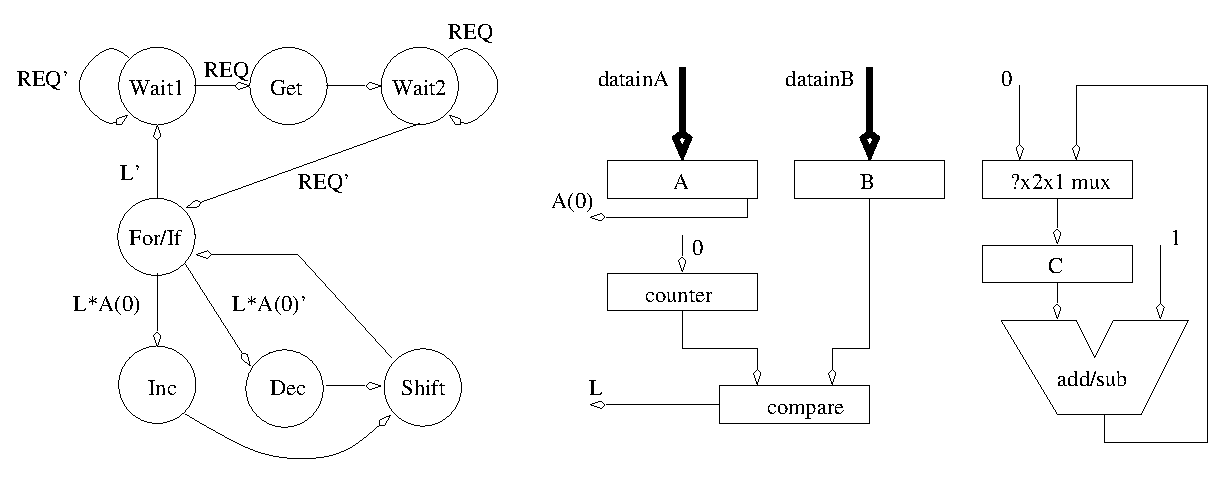
\includegraphics{./Fig3/dp&cu.eps}}

\begin{tabular}{|l||l|l|l|l|l|l|l|}  \hline
State & ACK & A       & B      & C      & Mux        & count   & Add/Sub \\ \hline
      & 0   & 00 hold & 0 hold & 0 hold & 0 pass 0   & 00 hold & 0 add \\ \hline
      & 1   & 01 SR   & 1 load & 1 load & 1 pass C$\pm$1 & 01 down & 1 sub \\ \hline
      &     & 10 SL   &        &        &            & 10 up   &       \\ \hline
      &     & 11 load &        &        &            & 11 load &       \\ \hline   \hline
Wait1 & \x  &         &        &        &            &         &       \\ \hline
Get   & \x  &  \x     &  \x    &  \x    &            &         &  \x   \\ \hline
Wait2 & \x  &  \x     &        &        &  \x        &  \x     &       \\ \hline
For/If &    &         &        &        &            &         &       \\ \hline
Inc   &     &  \x     &        &  \x    &  \x        &         & \x    \\ \hline
Dec   & \x  &         &        &  \x    &  \x        &         & \x    \\ \hline
Shift &     &  \x     &  \x    &  \x    &  \x        &         & \x    \\ \hline
\end{tabular}

\pagebreak
Questions 53-56 are based on the datapath and control shown on the previous page.

\item{\bf (2 pts.)} How many bits are in the status word?

\begin{tabular}{p{0.75in}p{0.75in}p{0.75in}p{0.75in}p{0.75in}}
a) 1 & b) 2 & c) 3 & d) 5 & e) 9 \\
\end{tabular}

\item{\bf (2 pts.)} How many bits are in the control word?

\begin{tabular}{p{0.75in}p{0.75in}p{0.75in}p{0.75in}p{0.75in}}
a) 2 & b) 3 & c) 5 & d) 7 & e) 9 \\
\end{tabular}

\item{\bf (3 pts.)} What is the Memory Input Equation for the For/If
flip flop; assume a ones-hot encoding?
\begin{description}
\item{a) } $D_{\rm For/If} = Q_{\rm Wait1}*L' + Q_{\rm Inc}*L*A(0) + Q_{\rm Dec}*L*A(0)'$
\item{b) } $Q_{\rm For/If} = D_{\rm Wait1}*L' + D_{\rm Inc}*L*A(0) + D_{\rm Dec}*L*A(0)'$
\item{c) } $D_{\rm For/If} = Q_{\rm Wait2}*REQ' + Q_{\rm Shift}$
\item{d) } $Q_{\rm For/If} = D_{\rm Wait2}*REQ' + D_{\rm Shift}$
\item{e) } None of the above.
\end{description}

\item{\bf (2 pts.)} Which of the following is the circuit playing in the
two-line handshake?
\begin{description}
\item{a) } Active Producer
\item{b) } Active Consumer
\item{c) } Passive Producer
\item{d) } Passive Consumer
\end{description}

\pagebreak
%% This is an ABET survey
%% Edited 12/2005 to include program outcomes
%% Edited 12/2008 to remove program outcomes

%% \begin{center} 
%% CSE 271 -- Introduction to Digital Systems \\
%% Course Objectives Survey \\ 
%% Penn State Erie, The Behrend College
%% \end{center}

\small{
In order to assure the continued success of the Behrend ECE
program, I would appreciate your evaluation of whether or
not this course met its learning objectives.  All answers
will be kept anonymous and will be used for the future 
improvement of this course and the entire ECE program.
Please record your answers on the SCANTRON form.
Thanks for your help.
}

\begin{tabular}{p{0.25in}p{2.5in}|p{0.45in}|p{0.4in}|p{0.4in}|p{0.4in}|p{0.4in}|} \\ \cline{3-7}
    &  & 
{\scriptsize Strongly Disagree} A & 
{\scriptsize Disagree} B & 
{\scriptsize Neutral} C & 
{\scriptsize Agree} D & 
{\scriptsize Strongly Agree} E \\ \hline

\item & I understand how to convert numbers from one base to another and 
how to add and subtract numbers represented in binary and 2's complement 
form. 
 & & & & & \\ \hline

\item & I understand how to convert between a truth table, a circuit diagram,
boolean expression and a word statement.
 & & & & & \\ \hline

\item & I understand how to simplify logic expression into SOP or
POS minimal form with or without don't cares.
 & & & & & \\ \hline

\item & I understand how to use ESPRESSO to minimize combinational logic
functions.
 & & & & & \\ \hline

\item & I understand how adders, comparators, multiplexers and decoders 
are built and how they operate. 
 & & & & & \\ \hline

\item & I understand how D,T,SR,JK, latches, clock latches and flip flops 
are supposed to operate. 
 & & & & & \\ \hline

\item & I understand how registers, shift registers, counters, tri-state 
logic and RAMs are built and how they should operate. 
 & & & & & \\ \hline

\item & I understand how to design Finite State Machines using a dense 
or Ones Hot encoding. 
 & & & & & \\ \hline

\item & I understand how to implement complex digital systems using the 
datapath and control design approach. 
 & & & & & \\ \hline

\end{tabular}

\end{enumerate}
\end{document}
